\section{Tikz}

\subsection{tikzpicture}

\subsubsection{Un grafico base}

\begin{verbatim}
    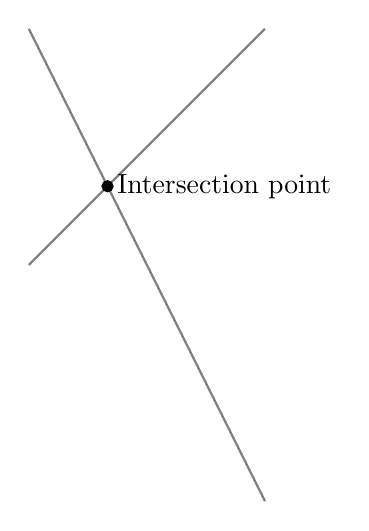
\begin{tikzpicture}
        \draw[gray, thick] (-1,2) -- (2,-4);
        \draw[gray, thick] (-1,-1) -- (2,2);
        \filldraw[black] (0,0) circle (2pt) node[anchor=west] {Intersection point};
    \end{tikzpicture}
\end{verbatim}

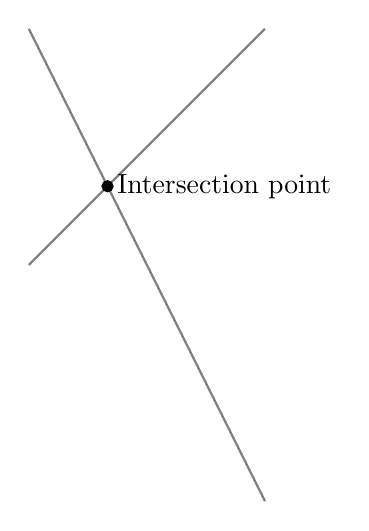
\begin{tikzpicture}
\draw[gray, thick] (-1,2) -- (2,-4);
\draw[gray, thick] (-1,-1) -- (2,2);
\filldraw[black] (0,0) circle (2pt) node[anchor=west] {Intersection point};
\end{tikzpicture}

\subsubsection{Albero MergeSort}

Per avere controllo sulle posizioni:

\begin{verbatim}
[level distance=1.5cm,
level 1/.style={sibling distance=3.5cm},
level 2/.style={sibling distance=1cm}]
\end{verbatim}

\begin{verbatim}
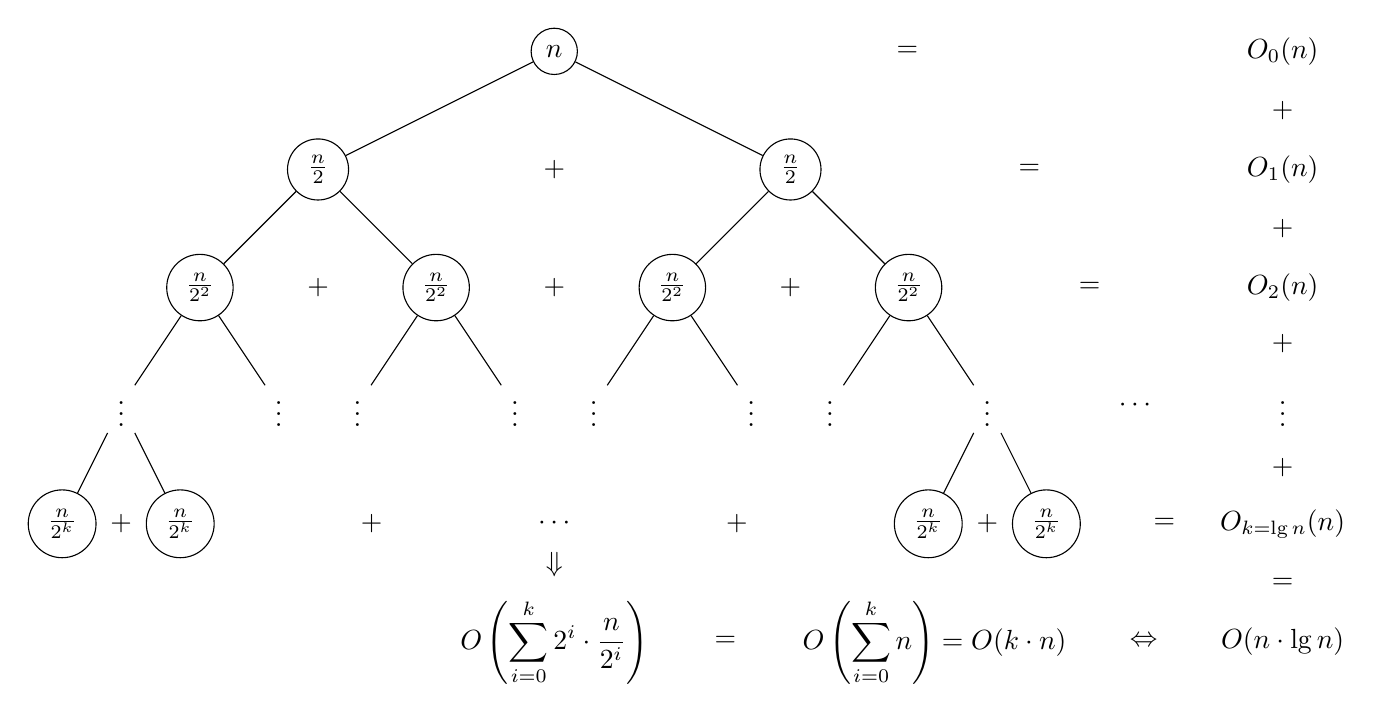
\begin{tikzpicture}[level/.style={sibling distance=60mm/#1}]
\node [circle,draw] (z){$n$}
  child {node [circle,draw] (a) {$\frac{n}{2}$}
    child {node [circle,draw] (b) {$\frac{n}{2^2}$}
      child {node {$\vdots$}
        child {node [circle,draw] (d) {$\frac{n}{2^k}$}}
        child {node [circle,draw] (e) {$\frac{n}{2^k}$}}
      } 
      child {node {$\vdots$}}
    }
    child {node [circle,draw] (g) {$\frac{n}{2^2}$}
      child {node {$\vdots$}}
      child {node {$\vdots$}}
    }
  }
  child {node [circle,draw] (j) {$\frac{n}{2}$}
    child {node [circle,draw] (k) {$\frac{n}{2^2}$}
      child {node {$\vdots$}}
      child {node {$\vdots$}}
    }
  child {node [circle,draw] (l) {$\frac{n}{2^2}$}
    child {node {$\vdots$}}
    child {node (c){$\vdots$}
      child {node [circle,draw] (o) {$\frac{n}{2^k}$}}
      child {node [circle,draw] (p) {$\frac{n}{2^k}$}
        child [grow=right] {node (q) {$=$} edge from parent[draw=none]
          child [grow=right] {node (q) {$O_{k = \lg n}(n)$} edge from parent[draw=none]
            child [grow=up] {node (r) {$\vdots$} edge from parent[draw=none]
              child [grow=up] {node (s) {$O_2(n)$} edge from parent[draw=none]
                child [grow=up] {node (t) {$O_1(n)$} edge from parent[draw=none]
                  child [grow=up] {node (u) {$O_0(n)$} edge from parent[draw=none]}
                }
              }
            }
            child [grow=down] {node (v) {$O(n \cdot \lg n)$}edge from parent[draw=none]}
          }
        }
      }
    }
  }
};
\path (a) -- (j) node [midway] {+};
\path (b) -- (g) node [midway] {+};
\path (k) -- (l) node [midway] {+};
\path (k) -- (g) node [midway] {+};
\path (d) -- (e) node [midway] {+};
\path (o) -- (p) node [midway] {+};
\path (o) -- (e) node (x) [midway] {$\cdots$}
  child [grow=down] {
    node (y) {$O\left(\displaystyle\sum_{i = 0}^k 2^i \cdot \frac{n}{2^i}\right)$}
    edge from parent[draw=none]
  };
\path (q) -- (r) node [midway] {+};
\path (s) -- (r) node [midway] {+};
\path (s) -- (t) node [midway] {+};
\path (s) -- (l) node [midway] {=};
\path (t) -- (u) node [midway] {+};
\path (z) -- (u) node [midway] {=};
\path (j) -- (t) node [midway] {=};
\path (y) -- (x) node [midway] {$\Downarrow$};
\path (v) -- (y)
  node (w) [midway] {$O\left(\displaystyle\sum_{i = 0}^k n\right) = O(k \cdot n)$};
\path (q) -- (v) node [midway] {=};
\path (e) -- (x) node [midway] {+};
\path (o) -- (x) node [midway] {+};
\path (y) -- (w) node [midway] {$=$};
\path (v) -- (w) node [midway] {$\Leftrightarrow$};
\path (r) -- (c) node [midway] {$\cdots$};
\end{tikzpicture}
\end{verbatim}
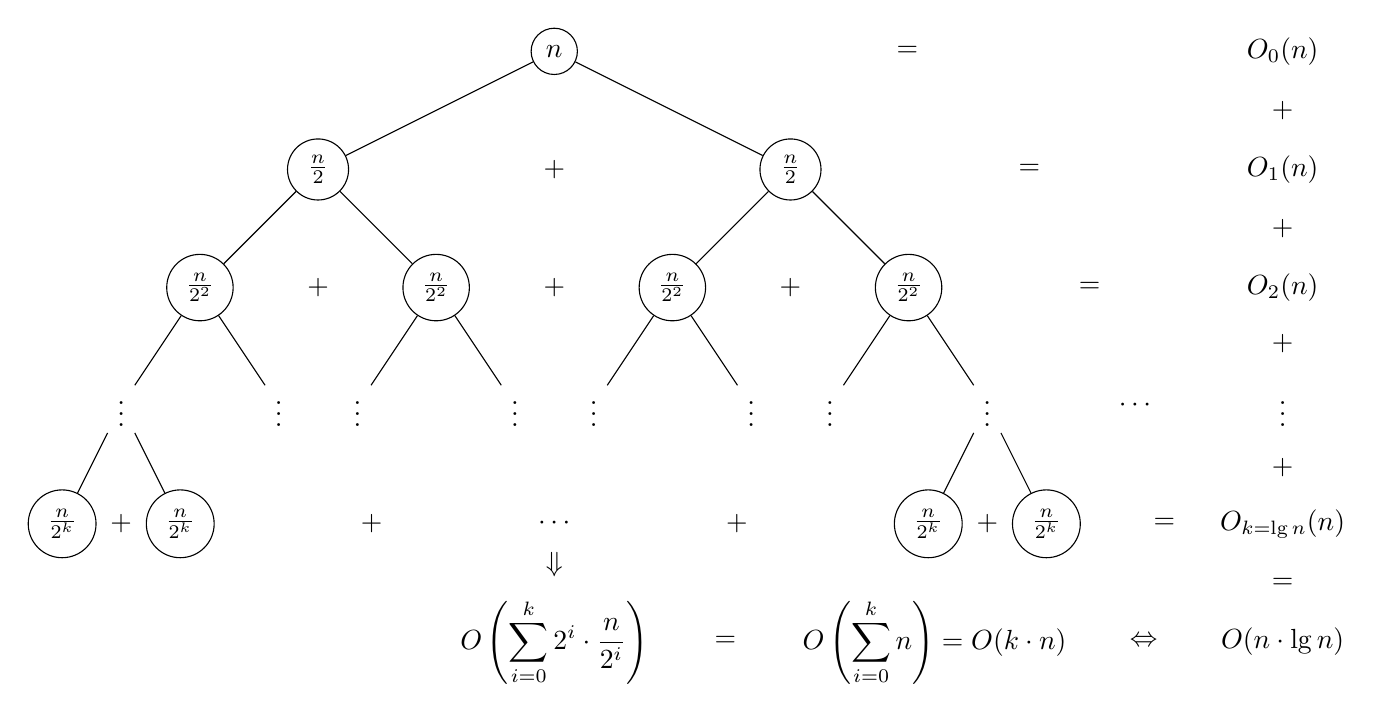
\begin{tikzpicture}[level/.style={sibling distance=60mm/#1}]
\node [circle,draw] (z){$n$}
  child {node [circle,draw] (a) {$\frac{n}{2}$}
    child {node [circle,draw] (b) {$\frac{n}{2^2}$}
      child {node {$\vdots$}
        child {node [circle,draw] (d) {$\frac{n}{2^k}$}}
        child {node [circle,draw] (e) {$\frac{n}{2^k}$}}
      } 
      child {node {$\vdots$}}
    }
    child {node [circle,draw] (g) {$\frac{n}{2^2}$}
      child {node {$\vdots$}}
      child {node {$\vdots$}}
    }
  }
  child {node [circle,draw] (j) {$\frac{n}{2}$}
    child {node [circle,draw] (k) {$\frac{n}{2^2}$}
      child {node {$\vdots$}}
      child {node {$\vdots$}}
    }
  child {node [circle,draw] (l) {$\frac{n}{2^2}$}
    child {node {$\vdots$}}
    child {node (c){$\vdots$}
      child {node [circle,draw] (o) {$\frac{n}{2^k}$}}
      child {node [circle,draw] (p) {$\frac{n}{2^k}$}
        child [grow=right] {node (q) {$=$} edge from parent[draw=none]
          child [grow=right] {node (q) {$O_{k = \lg n}(n)$} edge from parent[draw=none]
            child [grow=up] {node (r) {$\vdots$} edge from parent[draw=none]
              child [grow=up] {node (s) {$O_2(n)$} edge from parent[draw=none]
                child [grow=up] {node (t) {$O_1(n)$} edge from parent[draw=none]
                  child [grow=up] {node (u) {$O_0(n)$} edge from parent[draw=none]}
                }
              }
            }
            child [grow=down] {node (v) {$O(n \cdot \lg n)$}edge from parent[draw=none]}
          }
        }
      }
    }
  }
};
\path (a) -- (j) node [midway] {+};
\path (b) -- (g) node [midway] {+};
\path (k) -- (l) node [midway] {+};
\path (k) -- (g) node [midway] {+};
\path (d) -- (e) node [midway] {+};
\path (o) -- (p) node [midway] {+};
\path (o) -- (e) node (x) [midway] {$\cdots$}
  child [grow=down] {
    node (y) {$O\left(\displaystyle\sum_{i = 0}^k 2^i \cdot \frac{n}{2^i}\right)$}
    edge from parent[draw=none]
  };
\path (q) -- (r) node [midway] {+};
\path (s) -- (r) node [midway] {+};
\path (s) -- (t) node [midway] {+};
\path (s) -- (l) node [midway] {=};
\path (t) -- (u) node [midway] {+};
\path (z) -- (u) node [midway] {=};
\path (j) -- (t) node [midway] {=};
\path (y) -- (x) node [midway] {$\Downarrow$};
\path (v) -- (y)
  node (w) [midway] {$O\left(\displaystyle\sum_{i = 0}^k n\right) = O(k \cdot n)$};
\path (q) -- (v) node [midway] {=};
\path (e) -- (x) node [midway] {+};
\path (o) -- (x) node [midway] {+};
\path (y) -- (w) node [midway] {$=$};
\path (v) -- (w) node [midway] {$\Leftrightarrow$};
\path (r) -- (c) node [midway] {$\cdots$};
\end{tikzpicture}

% \begin{tikzpicture}[level/.style={sibling distance=60mm/#1}]
\begin{tikzpicture}[level/.style={sibling distance=40mm}]
    \node [draw, label=right:{Testo $math$}] (z){$n = f^{(0)}(n)$}
        child { node [ellipse,draw] (a) {$a f^{(0)}(n)$}
            child { node [circle,draw] (c) {$c f^{(0)}(n)$}
            }
            child { node [rectangle,draw] (d) {$d f^{(0)}(n)$}
                child { node [rectangle,draw] (e) {$e f^{(0)}(n)$}
                }
                child { node [rectangle,draw] (f) {$f f^{(0)}(n)$}
                }
            }
        }
        child { node [circle,draw] (b) {$b f^{(0)}(n)$}
        }
        % child [grow=right] {node (q) {$O_{k = \lg n}(n)$} edge from parent[draw=none]
        % }
    ;
\path (a) -- (b) node [midway] {$\cdots S(n) \cdots$ };
\end{tikzpicture}



\subsubsection{Grafo con archi evidenziati}

Info su
% https://www.overleaf.com/project/5dbc3071520a9e0001edc9f8
\href{https://www.overleaf.com/project/5dbc3071520a9e0001edc9f8}{overleaf}.

Stili locali alla figura
\href{https://tex.stackexchange.com/a/52379}{stackexchange}.
\begin{verbatim}
\begin{tikzpicture} [some options,
        first style/.style={blah},
        second style/.style={blub}
    ]
    ...
\end{tikzpicture}
\end{verbatim}

% Declare layers
\pgfdeclarelayer{background}
\pgfsetlayers{background,main}

\begin{figure}[h]
    \centering
    \caption{Algoritmo di Prim}
    \label{fig:prim1}
    %%%%%%%%%%%%%%%%%%%%%%%%%%%%%%%%%%%%%%%%%%%%%%%%%%%%%%%%%%%%%%%%%%%%%%%%%%%%%%%%%%%%%%%%%%
    \begin{subfigure}[b]{0.45\textwidth}
        \caption{Archi uscenti dal primo nodo}
        \label{fig:au1}
        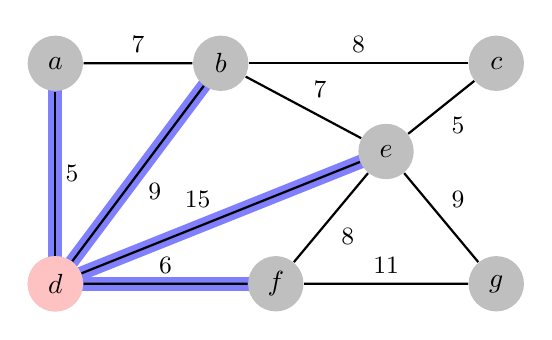
\begin{tikzpicture} [
                % automagically put labels not on edges
                auto,
                % exchanges the roles of left and right in automatic placement
                % the side the label is put on depends on the order of the nodes in the edge
                swap,
                scale=1.4,
                vertex/.style={circle,fill=black!25,minimum size=20pt,inner sep=0pt},
                selected vertex/.style = {vertex, fill=red!24},
                edge/.style = {draw,thick,-},
                weight/.style = {font=\small},
                selected edge/.style = {draw,line width=5pt,-,red!50},
                outbound edge/.style = {draw,line width=5pt,-,blue!50},
                ignored edge/.style = {draw,line width=5pt,-,black!20}
            ]
            % First we draw the vertices
            \foreach \pos/\name in {
            {(0,1)/a}, {(1.5,1)/b}, {(4,1)/c}, {(0,-1)/d}, {(3,0.2)/e}, {(2,-1)/f}, {(4,-1)/g}}
                \node[vertex] (\name) at \pos {$\name$};
            % Connect vertices with edges and draw weights
            \foreach \source/ \dest /\weight in {b/a/7, c/b/8, d/a/5, d/b/9,
                                                 e/b/7, e/c/5, e/d/15,
                                                 f/d/6, f/e/8, g/e/9, g/f/11}
                \path[edge] (\source) -- node[weight] {$\weight$} (\dest);
            % color a node
            % \path node[selected vertex] at (d) {$d$};
            % prepare it in loop version anyway
            \foreach \vertex in {d}
                \path node[selected vertex] at (\vertex) {$\vertex$};
            % For convenience we use a background layer to highlight edges
            % This way we don't have to worry about the highlighting covering
            % weight labels. 
            \begin{pgfonlayer}{background}
                \foreach \source / \dest in {d/a,d/b,d/e,d/f}
                    \path[outbound edge] (\source.center) -- (\dest.center);
            \end{pgfonlayer}
        \end{tikzpicture}
    \end{subfigure}
    \quad
    %%%%%%%%%%%%%%%%%%%%%%%%%%%%%%%%%%%%%%%%%%%%%%%%%%%%%%%%%%%%%%%%%%%%%%%%%%%%%%%%%%%%%%%%%%
    \begin{subfigure}[b]{0.45\textwidth}
        \caption{Arco selezionato}
        \label{fig:au2}
        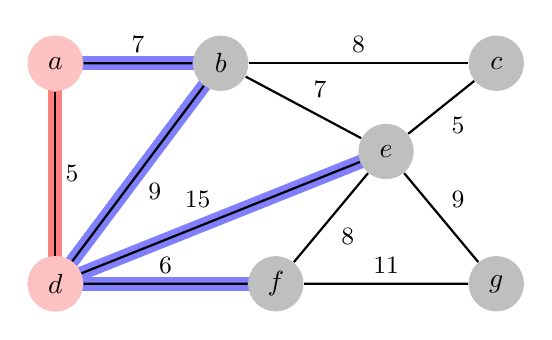
\begin{tikzpicture} [
                auto,
                swap,
                scale=1.4,
                vertex/.style={circle,fill=black!25,minimum size=20pt,inner sep=0pt},
                selected vertex/.style = {vertex, fill=red!24},
                edge/.style = {draw,thick,-},
                weight/.style = {font=\small},
                selected edge/.style = {draw,line width=5pt,-,red!50},
                outbound edge/.style = {draw,line width=5pt,-,blue!50},
                ignored edge/.style = {draw,line width=5pt,-,black!20}
            ]
            % First we draw the vertices
            \foreach \pos/\name in {
                {(0,1)/a}, {(1.5,1)/b}, {(4,1)/c}, {(0,-1)/d}, {(3,0.2)/e}, {(2,-1)/f}, {(4,-1)/g}}
                \node[vertex] (\name) at \pos {$\name$};
            % Connect vertices with edges and draw weights
            \foreach \source/ \dest /\weight in {b/a/7, c/b/8, d/a/5, d/b/9,
                                                 e/b/7, e/c/5, e/d/15,
                                                 f/d/6, f/e/8, g/e/9, g/f/11}
                \path[edge] (\source) -- node[weight] {$\weight$} (\dest);
            % color a node
            \foreach \vertex in {d,a}
                \path node[selected vertex] at (\vertex) {$\vertex$};
            \begin{pgfonlayer}{background}
                \foreach \source / \dest in {b/a,d/b,d/e,d/f}
                    \path[outbound edge] (\source.center) -- (\dest.center);
                \foreach \source / \dest in {d/a}
                    \path[selected edge] (\source.center) -- (\dest.center);
            \end{pgfonlayer}
        \end{tikzpicture}
    \end{subfigure}
    \\
    %%%%%%%%%%%%%%%%%%%%%%%%%%%%%%%%%%%%%%%%%%%%%%%%%%%%%%%%%%%%%%%%%%%%%%%%%%%%%%%%%%%%%%%%%%
    \begin{subfigure}[b]{0.45\textwidth}
        \caption{Secondo arco selezionato}
        \label{fig:au3}
        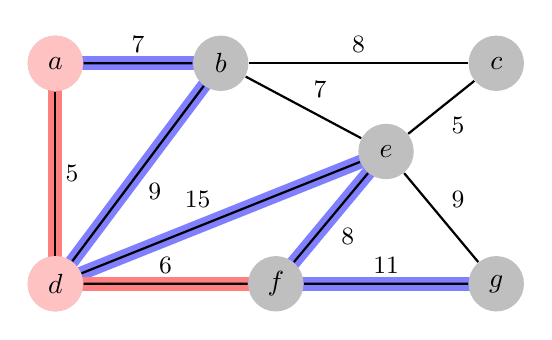
\begin{tikzpicture} [
                auto,
                swap,
                scale=1.4,
                vertex/.style={circle,fill=black!25,minimum size=20pt,inner sep=0pt},
                selected vertex/.style = {vertex, fill=red!24},
                edge/.style = {draw,thick,-},
                weight/.style = {font=\small},
                selected edge/.style = {draw,line width=5pt,-,red!50},
                outbound edge/.style = {draw,line width=5pt,-,blue!50},
                ignored edge/.style = {draw,line width=5pt,-,black!20}
            ]
            % First we draw the vertices
            \foreach \pos/\name in {
                {(0,1)/a}, {(1.5,1)/b}, {(4,1)/c}, {(0,-1)/d}, {(3,0.2)/e}, {(2,-1)/f}, {(4,-1)/g}}
                \node[vertex] (\name) at \pos {$\name$};
            % Connect vertices with edges and draw weights
            \foreach \source/ \dest /\weight in {b/a/7, c/b/8, d/a/5, d/b/9,
                                                 e/b/7, e/c/5, e/d/15,
                                                 f/d/6, f/e/8, g/e/9, g/f/11}
                \path[edge] (\source) -- node[weight] {$\weight$} (\dest);
            % color a node
            \foreach \vertex in {d,a}
                \path node[selected vertex] at (\vertex) {$\vertex$};
            \begin{pgfonlayer}{background}
                \foreach \source / \dest in {b/a,d/b,d/e,e/f,f/g}
                    \path[outbound edge] (\source.center) -- (\dest.center);
                \foreach \source / \dest in {d/a, d/f}
                    \path[selected edge] (\source.center) -- (\dest.center);
            \end{pgfonlayer}
        \end{tikzpicture}
    \end{subfigure}
    \quad
    %%%%%%%%%%%%%%%%%%%%%%%%%%%%%%%%%%%%%%%%%%%%%%%%%%%%%%%%%%%%%%%%%%%%%%%%%%%%%%%%%%%%%%%%%%
    \begin{subfigure}[b]{0.45\textwidth}
        \caption{Terzo arco selezionato}
        \label{fig:au4}
        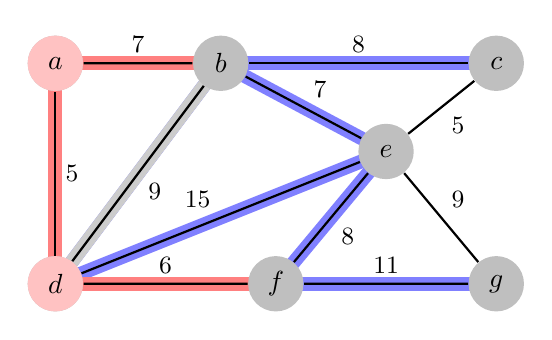
\begin{tikzpicture} [
                auto,
                swap,
                scale=1.4,
                vertex/.style={circle,fill=black!25,minimum size=20pt,inner sep=0pt},
                selected vertex/.style = {vertex, fill=red!24},
                edge/.style = {draw,thick,-},
                weight/.style = {font=\small},
                selected edge/.style = {draw,line width=5pt,-,red!50},
                outbound edge/.style = {draw,line width=5pt,-,blue!50},
                ignored edge/.style = {draw,line width=5pt,-,black!20}
            ]
            % First we draw the vertices
            \foreach \pos/\name in {
                {(0,1)/a}, {(1.5,1)/b}, {(4,1)/c}, {(0,-1)/d}, {(3,0.2)/e}, {(2,-1)/f}, {(4,-1)/g}}
                \node[vertex] (\name) at \pos {$\name$};
            % Connect vertices with edges and draw weights
            \foreach \source/ \dest /\weight in {b/a/7, c/b/8, d/a/5, d/b/9,
                                                 e/b/7, e/c/5, e/d/15,
                                                 f/d/6, f/e/8, g/e/9, g/f/11}
                \path[edge] (\source) -- node[weight] {$\weight$} (\dest);
            % color a node
            \foreach \vertex in {d,a}
                \path node[selected vertex] at (\vertex) {$\vertex$};
            \begin{pgfonlayer}{background}
                \foreach \source / \dest in {d/b,d/e,e/f,f/g,b/e,b/c}
                    \path[outbound edge] (\source.center) -- (\dest.center);
                \foreach \source / \dest in {d/a, d/f, a/b}
                    \path[selected edge] (\source.center) -- (\dest.center);
                \foreach \source / \dest in {d/b}
                    \path[ignored edge] (\source.center) -- (\dest.center);
            \end{pgfonlayer}
        \end{tikzpicture}
    \end{subfigure}
\end{figure}

